\documentclass[11pt]{article}
\usepackage[utf8]{inputenc}
\usepackage[english]{babel}
\usepackage{bilal2vec}

\title{SE 380 — Midterm Review}
\author{Bilal Khan\\
\href{mailto:bilal2vec@gmail.com}{bilal2vec@gmail.com}}
\date{\today}

\begin{document}

\maketitle

\tableofcontents

\section{Assignment 1}

\subsection{Question 1}

\subsubsection{a}

\[ x = \begin{bmatrix} x_1 \\ x_2 \end{bmatrix} = \begin{bmatrix} \theta \\ \dot{\theta} \end{bmatrix} \]
\[ u = \tau \]
\[ J \ddot{\theta} + \dfrac{mgl}{2} \sin \theta = \tau \]

\[ J \ddot{\theta} + \dfrac{mgl}{2} \sin \theta = u \]

\begin{align*}
    \begin{bmatrix}
        \dot{x_1} \\
        \dot{x_2} \\
    \end{bmatrix}
    &=
    \begin{bmatrix}
        x_2 \\
        \dfrac{u}{J} - \dfrac{mgl}{2J} \sin x_1 \\
    \end{bmatrix}
\end{align*}

With the required approximation of $\sin x = x$ to show this in matrix form, this is given by:

\[ \dot{x}(t) = A x(t) + Bu(t) \]

\[
\begin{bmatrix}
    \dot{x_1}(t) \\
    \dot{x_2}(t) \\
\end{bmatrix}
=
\begin{bmatrix}
    0 & 1 \\
    - \dfrac{mgl}{2J} & 0 \\
\end{bmatrix}
\begin{bmatrix}
    x_1(t) \\
    x_2(t) \\
\end{bmatrix}
+
\begin{bmatrix}
    0 \\
    \dfrac{1}{J} \\
\end{bmatrix}
u(t)
\]

\subsubsection{b}

The system is at its equilibrium points when $\dot{x}(t) = 0$. Therefore, we have that 

\[
\dot{x}(t) = 
\begin{bmatrix}
    0 \\
    0 \\
\end{bmatrix}
=
\begin{bmatrix}
    \dot{\theta} \\
    \ddot{\theta} \\
\end{bmatrix}
\]

Plugging this into our original equation, we have that

\[ J (0) + \dfrac{mgl}{2} \sin \theta = u \]
\[\sin\theta = \dfrac{2u}{mgl} \]

Equilibrium will happen at all points where $\sin \theta = \frac{2u}{mgl}$

\subsubsection{c}

The system is at an equilibrium point for state $\bar{x} = \begin{bmatrix} 0 \\ 0 \\ \end{bmatrix}$ and and input $\bar{u} = 0$.

We can linearalize the system around this point by taking the Jacobian of $\dot{x}$ with respect to $x$ and $u$.

\[
    A = 
    \begin{bmatrix}
        \dfrac{\partial \dot{x_1}}{\partial x_1} & \dfrac{\partial \dot{x_1}}{\partial x_2} \\
        \dfrac{\partial \dot{x_2}}{\partial x_1} & \dfrac{\partial \dot{x_2}}{\partial x_2} \\
    \end{bmatrix}
    = \begin{bmatrix}
        0 & 1 \\
        - \dfrac{mgl}{2J} \cos x_1 & 0 \\
    \end{bmatrix}
    = \begin{bmatrix}
        0 & 1 \\
        - \dfrac{mgl}{2J} \cos (0) & 0 \\
    \end{bmatrix}
    = \begin{bmatrix}
        0 & 1 \\
        - \dfrac{mgl}{2J} & 0 \\
    \end{bmatrix}
\]

\[
    B =
    \begin{bmatrix}
        \dfrac{\partial \dot{x_1}}{\partial u} \\
        \dfrac{\partial \dot{x_2}}{\partial u} \\
    \end{bmatrix}
    = \begin{bmatrix}
        0 \\
        \dfrac{1}{J} \\
    \end{bmatrix}
\]

The linearalized system is given by the general expression

\[ \dot{x} \approx \dot{x}(\bar{x}, \bar{u}) + A (x - \bar{x}) + B (u - \bar{u}) \]
\[ \dot{x} \approx A(x) + B (u) \]
\[
    \dot{x} \approx
    \begin{bmatrix}
        0 & 1 \\
        - \dfrac{mgl}{2J} & 0 \\
    \end{bmatrix}
    x +
    \begin{bmatrix}
        0 \\
        \dfrac{1}{J} \\
    \end{bmatrix}
    u
\]

\subsubsection{d}

The system is at equilibrium for $\bar{x} = \begin{bmatrix} \pi / 4 \\ 0 \\ \end{bmatrix}$ and $\bar{u} = \dfrac{mgl}{2\sqrt{2}}$.

We can again linearalize the system around this point by taking the Jacobian of $\dot{x}$ with respect to $x$ and $u$.

\[
    A =
    \begin{bmatrix}
        \dfrac{\partial \dot{x_1}}{\partial x_1} & \dfrac{\partial \dot{x_1}}{\partial x_2} \\
        \dfrac{\partial \dot{x_2}}{\partial x_1} & \dfrac{\partial \dot{x_2}}{\partial x_2} \\
    \end{bmatrix}
    = \begin{bmatrix}
        0 & 1 \\
        - \dfrac{mgl}{2J} \cos x_1 & 0 \\
    \end{bmatrix}
    = \begin{bmatrix}
        0 & 1 \\
        - \dfrac{mgl}{2J} \cos (\pi / 4) & 0 \\
    \end{bmatrix}
    = \begin{bmatrix}
        0 & 1 \\
        - \dfrac{mgl}{2J \sqrt 2} & 0 \\
    \end{bmatrix}
    = \begin{bmatrix}
        0 & 1 \\
        - \dfrac{mgl}{2 \sqrt 2 J} & 0 \\
    \end{bmatrix}
\]

\[
    B =
    \begin{bmatrix}
        \dfrac{\partial \dot{x_1}}{\partial u} \\
        \dfrac{\partial \dot{x_2}}{\partial u} \\
    \end{bmatrix}
    = \begin{bmatrix}
        0 \\
        \dfrac{1}{J} \\
    \end{bmatrix}
\]

The linearalized  system is given by the general expression

\[ \dot{x} \approx \dot{x}(\bar{x}, \bar{u}) + A (x - \bar{x}) + B (u - \bar{u}) \]
\[ \dot{x} \approx A(x - \bar{x}) + B (u - \bar{u}) \]
\[
    \dot{x} \approx
    \begin{bmatrix}
        0 & 1 \\
        - \dfrac{mgl}{2 \sqrt 2 J} & 0 \\
    \end{bmatrix}
    (x - \bar{x}) +
    \begin{bmatrix}
        0 \\
        \dfrac{1}{J} \\
    \end{bmatrix}
    (u - \bar{u})
\]

\subsubsection{e}

The system is at equilibrium at part (c) and at part (d) when it is at a 45 degree angle with the horizontal so I would use part (c)'s linearalized system to approximate the behavior of the system around the equilibrium point close to its initial conditions and part (d)'s linearlization when it is in equilibrium close to its initial conditions.

\subsection{Question 2}

\subsubsection{a}

\begin{minted}{python}
    import numpy as np
    import matplotlib.pyplot as plt

    def sim(delta_t, T, l, x, u):
        t = 0
        path = [x[:2]] # store p_x and p_y for bike path

        while t <= T:
            p_x, p_y, theta, v, delta = x[0], x[1], x[2], x[3], x[4]
            a, w = u(t)
            x_dot = np.array([
                v * np.cos(theta),
                v * np.sin(theta),
                (v / l) * np.tan(delta),
                a,
                w
            ])

            x = x + delta_t * x_dot
            t = t + delta_t

            p_x_prime, p_y_prime = x[0], x[1]
            path += [[p_x_prime, p_y_prime]]
        
        return np.array(path)
\end{minted}

\subsubsection{b}

\begin{minted}{python}
    import numpy as np
    import matplotlib.pyplot as plt

    delta_t = 0.01
    T = 10
    l = 2
    x = np.zeros(5)
    u = lambda t: (0.1, np.cos(t))

    path = sim(delta_t, T, l, x, u)
    
    plt.plot(path[:, 0], path[:, 1], label="Bike kinematic dynamics")
    plt.title("Path of bicycle")
    plt.xlabel("p_x")
    plt.ylabel("p_y")
    plt.legend()
    plt.show()
\end{minted}

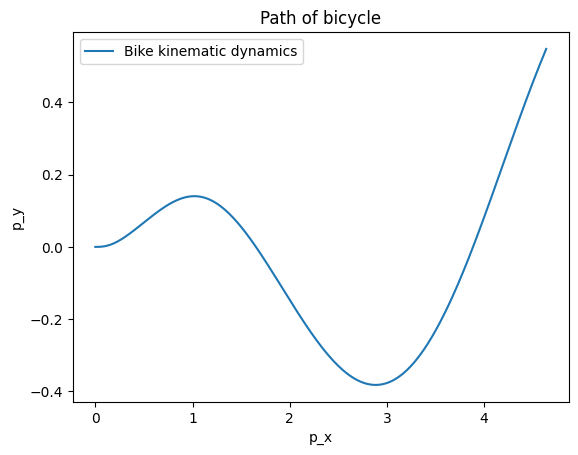
\includegraphics{a1.png}

\section{Assignment 2}

\subsection{Question 1}

\subsubsection{a}

Considering the state space model

\begin{align*}
    \dot{x} &= Ax + Bu \\
    y &= Cx + Du
\end{align*}

where $x \in \mathbb{R}^2$, $u \in \mathbb{R}^2$, and $y \in \mathbb{R}$, find values for $A, B, C, D$ such that the corresponding transfer function is

\begin{align*}
    G(s) &= \dfrac{\mu}{1 + \tau s} \\
\end{align*}

Taking the Laplace transform of the above equations, we get

\begin{align*}
    sX(s) - x(0) &= AX(s) + BU(s) \\
    Y(s) &= CX(s) + DU(s)
\end{align*}

Solving this, assuming initial state is zero, we get

\begin{align*}
    sX(s) - x(0) &= AX(s) + BU(s) \\
    sX(s) - AX(s) &= BU(s) \\
    X(s) (sI - A) &= BU(s) \\
    X(s) &= \dfrac{BU(s)}{sI - A} \\
    Y(s) &= \left( \dfrac{CB}{sI - A} + D \right) U(s) \\
    H(S) &= \dfrac{Y(s)}{U(s)} = \dfrac{CB}{sI - A} + D \\
    \dfrac{CB}{sI - A} &= \dfrac{\mu}{1 + \tau s} \\
    \dfrac{1}{\tau} \dfrac{CB}{sI - A} &= \dfrac{\mu}{1 + \tau s}
\end{align*}

We want $CB = \mu \tau$, so one possible solution is

\[
    C = \begin{bmatrix} \mu \tau & 0 \end{bmatrix} \\
    B = \begin{bmatrix} 1 \\ 0 \end{bmatrix}
\]

The $s + 1 / \tau$ term in $sI - A$ can be made simpler by dividing the left-hand side of the expression above by $1 / \tau$ to get $s + \frac{1}{\tau}$ in the denominator of the transfer function, and we want the same $x_1(t)$ state value to change as in $B$ so we want $A$ to be

\[
    A = \begin{bmatrix}
        -\dfrac{1}{\tau} & 0 \\
        0 & 0 \\ 
    \end{bmatrix}
\]

$D$ is zero because we do not use it in the transfer function.

\subsubsection{b}

No, there are multiple ways to set up the state space matrices to get the same transfer function. For example, we could have chosen $x_2(t)$ to be the state variable we use and then choose $C$ to be $\begin{bmatrix} 0 & \mu \tau \end{bmatrix}$ and $B$ to be $\begin{bmatrix} 0 \\ 1 \end{bmatrix}$, and $A$ to be $\begin{bmatrix} 0 & 0 \\ -\dfrac{1}{\tau} & 0 \end{bmatrix}$, and $D$ to be zero. This would have given us the same transfer function.

\subsection{Question 2}

\subsubsection{a}

Consider a first-order system with transfer function given by $H(s) = \dfrac{\mu}{1 + \tau s}$. Compute the response $y_1(t)$ to a step input $u_1(t) = H(t)$ and the response of $y_2(t)$ to a ramp input $u_2(t) = tHTt)$.

The laplace transform of $u_1(t)$ is $U_1(s) = \dfrac{1}{s}$ and the Laplace transform of $u_2(t)$ is $U_2(s) = \dfrac{1}{s^2}$

\begin{align*}
    Y_1(s) &= H(s) U_1(s) \\
     &= \dfrac{\mu}{1 + \tau s} \dfrac{1}{s} \\
     &= \dfrac{\mu}{s(1 + \tau s)} \\
    Y_2(s) &= H(s) U_2(s) \\
    &= \dfrac{\mu}{1 +\tau s} \dfrac{1}{s^2} \\
    &= \dfrac{\mu}{s^2(1 + \tau s)} \\
\end{align*}

We can compute the inverse Laplace transforms on their partial fraction decompositons.

\begin{align*}
    Y_1(s) &= \dfrac{\mu}{s(1 + \tau s)} \\
    \dfrac{\mu}{s(1 + \tau s)} &= \dfrac{A}{s} + \dfrac{B}{1 + \tau s} \\
    \mu &= A(1 + \tau s) + Bs \\
    \mu &= A \tag{s = 0} \\ 
    \mu &= \mu (1 + \tau s) + Bs \\
    \mu &= \mu + \mu \tau s + Bs \\
    0 &= s (\mu \tau + B) \tag{$s \neq 0$} \\
    B &= -\mu \tau \\
    Y_1(s) &= \dfrac{\mu}{s} - \dfrac{\mu \tau}{1 + \tau s} \\
    y_1(t) &= (\mu - \mu e^{-t / \tau}) u_1(t) \\
\end{align*}

\begin{align*}
    Y_2(s) &= \dfrac{\mu}{s^2(1 + \tau s)} \\
    \dfrac{\mu}{s^2(1 + \tau s)} &= \dfrac{A}{s} + \dfrac{B}{s^2} + \dfrac{C}{1 + \tau s} \\
    \mu &= A s(1 + \tau s) + B(1 + \tau s) + Cs^2 \\
    \mu &= B \tag{$s = 0$} \\
    \mu &= A s (1 + \tau s) + \mu (1 + \tau s) + Cs^2 \\
    \mu &= C (-1/\tau)^2 \tag{$s = -1/\tau$} \\
    \mu &= C / \tau^2 \\
    C &= \mu \tau^2 \\
    \mu &= As(1 + \tau s) + \mu (1 + \tau s) + \mu \tau^2 s^2 \\
    \mu &= As(1 + \tau s) + \mu + \mu \tau s + \mu \tau^2 s^2 \\
    0 &= As (1 + \tau s) + (1 + \tau s) \mu \tau s \\
    - (1 + \tau s) \mu \tau s &= As (1 + \tau s) \\
    - \mu \tau &= A \\
    Y_2(s) &= \dfrac{-\mu \tau}{s} + \dfrac{\mu}{s^2} + \dfrac{\mu \tau^2}{1 + \tau s} \\
    y_2(t) &= (-\mu \tau + \mu t + \mu \tau e^{-t / \tau}) u_2(t) \\ 
\end{align*}

\subsubsection{b}

\subsubsection{i}

$u_1(t)$ is positive and $1$ for all values $\geq 1$ so its value is fixed. As $t \to \infty$, $y_1(t) \to \mu$ for all values of $t$ and so the limit goes to $1$. For the abs of the difference to go to zero, we need $\mu = 1$.

\subsubsection{ii}

$u_2(t)$ is positive and $t$ for all values $t \geq 1$. As $t \to \infty$, the terms in

\[ | -\mu\tau + \mu t + \mu \tau e^{-t/\tau} - t | \]

go to

\[ | -\mu \tau + t (\mu - 1) | \]

This goes to zero as $t \to \infty$ if $\mu = 1$ and $\tau = 0$.

The first example is about tracking the error between a constant reference given by the input (a constant value of $1$ from the heaviside function) and so our system's error will go to zero if the gain of our transfer function $\mu$ is also one.

The second example is about tracking the error between a ramp reference with a slope of $t$ given by the input (the ramp) and so our system's error will go to zero if the gain of our transfer function $\mu$ is one and the time constant $\tau$ is zero. Setting $\mu$ to one ensures that the middle term in our response tracks the input and leads to zero error. However, this is \textit{probably} a case that is not physically feasible since that would mean that the damped exponential in our response would immediately go to zero. In more ,realistic cases, we would still set $\mu$ to one but we would set $\tau$ to a small value so that the damped exponential would go to zero quickly and the first term $\mu \tau$ would also reduce the error to a constant $\tau$ value.

\subsection{Question 3}

\subsubsection{a}

Given the equation $y(t) = u(t - \tau)$ where $\tau > 0$, its Laplace transform is $Y(s) = e^{-\tau s} U(s)$. Its transfer function is given by $H(s) = e^{-s \tau}$

\subsubsection{b}

$H(j\omega) = e^{-j \omega \tau}$. The magnitude in decibels is given by $20 \log_{10} |H(j\omega)| = 20 \log_{10} |e^{-j \omega \tau}| = 20 \log_{10} 1 = 0$. The angle is given by $\angle H(j\omega) = \angle e^{-j \omega \tau} = -\omega \tau$.

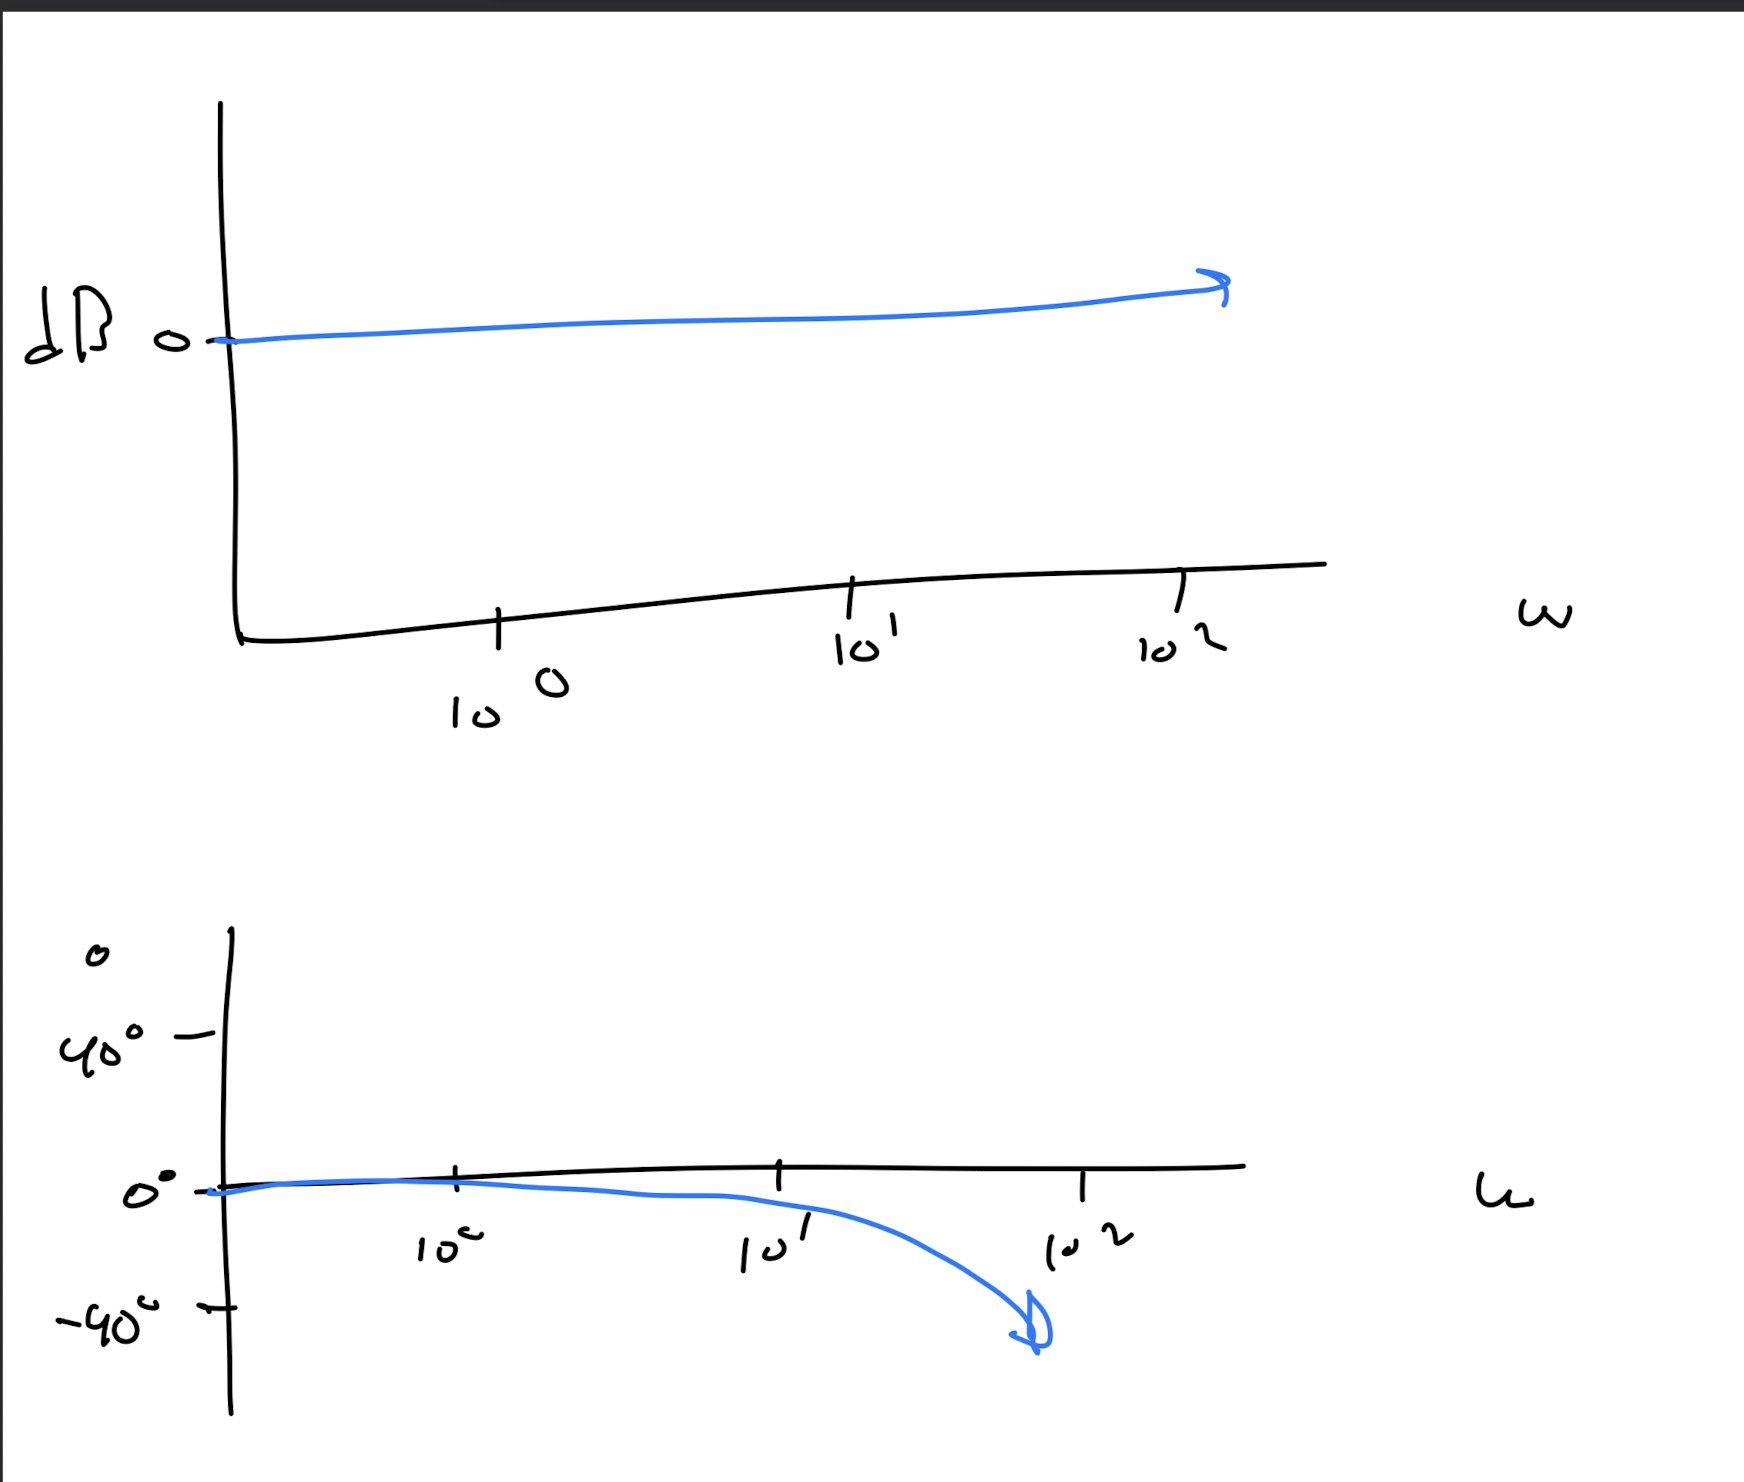
\includegraphics[width=300pt]{a2_q3.png}

\subsubsection{c}

$H(s) = e^{-\tau / s}$. Taking the Laplace transform of the input, $U(s) = \dfrac{0.15 \times 2 \pi}{s^2 + (2\pi)^2}$. The output is given by $Y(s) = H(s) U(s) = \dfrac{0.15 \times 2 \pi e^{-\tau / s}}{s^2 + (2\pi)^2}$. Taking the inverse Laplace transform, we get apply the rules for sin and time shifting to get $y(t) = 0.15 \times \sin (2\pi (t - \tau))$.

\subsubsection{d}

Yes it holds because the output is a sinusoid with a modified amplitude that has been phase shifted, but at the same frequency.

\section{E2.4}

A laser printer uses a laser beam to print copy rapidly for a computer. The laser is positioned by a control input \( r(t) \), so that we have

\begin{align*}
Y(s) = \frac{6(s + 50)}{s^2 + 40s + 300} R(s)
\end{align*}

The input $r(t)$ represents the desired position of the laser beam.

\begin{enumerate}
    \item If $r(t)$ is a unit step input, find the output $y(t)$.
    
    \begin{align*}
        Y(s) &= \dfrac{6(s + 50)}{(s + 30)(s + 10)} R(s) \\
        &= \dfrac{6(s + 50)}{(s + 30)(s + 10)} \dfrac{1}{s} \\
        &= \dfrac{A}{s} + \dfrac{B}{s + 30} + \dfrac{C}{s + 10}\\
        6(s + 50) &= A (s + 30) (s + 10) + B (s) (s + 10) + C (s) (s + 30)\\
        6(50) &= A (30)(10) \tag{$s = 0$} \\
        A &= 1 \\
        6(-30 + 50) &= B (-30) (-30 + 10) \tag{$s = -30$} \\
        6(20) &= B (-30) (-20) \\
        120 &= 600 B \\
        B &= 0.2 \\
        6(-10 + 50) &= C (-10) (-10 + 30) \tag{$s = -10$} \\
        6(40) &= C (-10) (20) \\
        240 &= -200 C \\
        C &= -1.2 \\
        y(t) &= 1 + 0.2 e^{-30t} - 1.2 e^{-10t}
    \end{align*}

    \item What is the final value of $y(t)$?
    
    $\lim_{t \xrightarrow{} \infty} y(t) = 1$.

\end{enumerate}
    
\section{E2.22}

\begin{align*}
    \dfrac{\omega(s)}{1/s} &= \dfrac{2(s + 4)}{(s + 5)(s + 1)^2} \\
    \omega(s) &= \dfrac{2(s + 4)}{s(s + 5)(s + 1)^2} \\
    \omega(s) &= \dfrac{A}{s} + \dfrac{B}{s + 5} + \dfrac{C}{s + 1} + \dfrac{D}{(s + 1)^2} \\
    2(s + 4) &= A (s + 5) (s + 1)^2 + B (s) (s + 1)^2 + C (s) (s + 5) (s + 1) + D (s) (s + 5) \\
    2(4) &= A (5)(1)^2 \xrightarrow{} A = \dfrac{8}{5} = 1.6 \tag{$s = 0$} \\
    2(-5 + 4) &= B (-5) (-5 + 1)^2 \xrightarrow{} 2(-1) = B (-5) (-4)^2 \tag{$s = -5$}\\
    B &= -2 / 16 * -5 \xrightarrow{} B = 0.025 \\
    2 (-1 + 4) &= D (-1) (-1 + 5) \xrightarrow{} 6 = D (-1) (4) \xrightarrow{} D = - 6 / 4 = -1.5 \tag{$s = -1$} \\
    2 (1 + 4) &= 1.6 (1 + 5) (1 + 1)^2 + (0.025) (1) (1 + 1)^2 + C (1) (1 + 5) (1 + 1) + (-1.5) (1) (1 + 5) \tag{$s = 1$} \\
    2(5) &= 1.6 (6) (4) + (0.025) (4) + C (6) (2) + (-1.5) (6) \\
    10 &= 1.6 (24) + (0.025) (4) + 12 C + (-1.5) (6) \\
    12 C &= 10 - 1.6 * 24 - 0.025 * 4 + 1.5 * 6 \\
    C &= (10 - 1.6 * 24 - 0.025 * 4 + 1.5 * 6) / 12 = -1.625 \\
    \omega(t) &= 1.6 + 0.025 e^{-5t} - 1.625 e^{-5} - 1.5 t e^{-t}
\end{align*}

\section{P2.4}

A nonlinear amplifier can be described by the following characteristic:

\begin{align*}
    v_0(t) &= \begin{cases}
        v_{in}^2  & v_{in} \geq 0 \\
        -v_{in}^2 & v_{in} < 0 \\
    \end{cases}
\end{align*}

The amplifier will be operated over a range of $\pm0.5$V around the operating point for $v_{in}$. Describe the amplifier by a linear approximation (a) when the operating point is $v_{in} = 0$ and (b) when the oeprating point is $v_{in} = 1V$. Obtain a sketch of the nonlinear function and the approximation for each case. 

\begin{enumerate}
    \item $v_0(t) \approx v_0(0) + \dfrac{dv_0}{dv_{in}} (0) (t - 0) = 0 + 2(0)(t - 0) = 0$
    \item $v_(t) \approx v_0(1) + \dfrac{dv_0}{dv_{in}} (1) (t - 1) = 1 + 2(1) (t - 1) = 2t - 1$ 
\end{enumerate}

\section{P2.36}

A system is represented by $Y(s) = \frac{30}{s^3 + 9s^2 + 26s + 30} R(s)$ (a) Determine the partial fraction expansion and $y(t)$ for a ramp input $r(t) = t, t \geq 0$. (b) Obtain a plot of $y(t)$ for part (a), and find $y(t)$ for $t = 1.0$s. (c) Determine the impuluse response of the system $y(t)$ for $t \geq 0$. (d) Obtain a plot of $y(t)$ for part (c) and find $y(t)$ for $t = 1.0$s.

Similar to above, but with a more annoying decomposition. Not doing by hand. Impulse response is given by the inv laplace transform of the transfer fn, the ramp input in laplace space is $1/s^2$.

\section{E3.2}

A robot arm drive system for one joint can be represented by the differential equation

\[ \dfrac{dv(t)}{dt} = -k_1 v(t) - k_2 y(t) + k_3 i(t) \]

where $v(t)$ is velocity, $y(t)$ is position, and $i(t)$ is the control motor current. Put the equations in state variable form and setup the matrix form for $k_1 = k_2 = 1$.

\begin{align*}
    \dfrac{d}{dt} \left(
        \begin{bmatrix}
            v(t) \\
            y(t) \\
        \end{bmatrix}
    \right)
    =
    \begin{bmatrix}
        -k_1 & -k_2 \\
        1 & 0 \\
    \end{bmatrix}
    \begin{bmatrix}
        v(t) \\
        y(t) \\
    \end{bmatrix}
    +
    \begin{bmatrix}
        k_3 \\
        0 \\
    \end{bmatrix}
    i(t)
\end{align*}

\section{E3.3}

A system can be represented by the state vector differential equation $\dot x(t) = Ax(t) + Bu(t)$ where $A = \begin{bmatrix} 0 & 1 \\ -1 & -2 \\ \end{bmatrix}$ Find the characteristic roots of the system.

\begin{align*}
    \det(\lambda I - A) = \det \begin{bmatrix}
        \lambda & -1 \\
        1 & \lambda + 2 \\
    \end{bmatrix}
    = \lambda (\lambda + 2) - (-1) (1) = \lambda^2 + 2 \lambda + 1 = (\lambda + 1)^2
\end{align*}

The roots are $-1$ with multiplicity two.

\section{E3.4}

Obtain a state variable matrix for a system with a differential equation

\[ \dfrac{d^3 y(t)}{dt^3} + 4 \dfrac{d^2 y(t)}{dt^2} + 6 \dfrac{dy(t)}{dt} + 8 y(t) = 20 u(t) \]

Lets use the state variables $x_1(t) = y(t)$, $x_2(t) = \frac{dy(t)}{dt}$, and $x_3(t) = \frac{d^2 y(t)}{dt^2}$. Then we can write our system as

\begin{align*}
    \begin{bmatrix}
        \frac{d x_1(t)}{dt} \\
        \frac{d x_2(t)}{dt} \\
        \frac{d x_3(t)}{dt} \\
    \end{bmatrix}
    =
    \begin{bmatrix}
        x_2(t) \\
        x_3(t) \\
        -4 x_3(5) - 6 x_2(t) - 8 x_1(t) + 20 u(t) \\
    \end{bmatrix}
\end{align*}

In $\dot x(t) = Ax(t) + Bu(t)$ form, we have

\[
\begin{bmatrix}
    \dot x_1(t) \\
    \dot x_2(t) \\
    \dot x_3(t) \\
\end{bmatrix}
=
\begin{bmatrix}
    0 & 1 & 0 \\
    0 & 0 & 1 \\
    -8 & -6 & -4 \\
\end{bmatrix}
\begin{bmatrix}
    x_1(t) \\
    x_2(t) \\
    x_3(t) \\
\end{bmatrix}
+
\begin{bmatrix}
    0 \\
    0 \\
    20 \\
\end{bmatrix}
u(t)
\]

\[
y = \begin{bmatrix}
    1 & 0 & 0 \\
\end{bmatrix}
\begin{bmatrix}
    x_1(t) \\
    x_2(t) \\
    x_3(t) \\
\end{bmatrix}
\]

\section{E3.6}

Consider the system $\dot x(t) = \begin{bmatrix} 0 & 1 \\ 0 & 0 \\ \end{bmatrix} \dot x(t)$. Find the state transition matrix $\phi(t)$ and for the initial conditions $x_1(0) = x_2(0) = 1$, find $x(t)$.

The state transition matrix is a matrix whose product with the state vector at time $t_0$ gives the state vector at time $t$. It is given by the matrix exponential of the matrix $A$, $\phi(t) = e^{At}$. For $2\times2$ matrices, it can be found by computing $e^{At} = I + At + \frac{1}{2!} (At)^2 + \frac{1}{3!} (At)^3 + \dots$. Note that $A^2$ is the zero matrix and all powers of $A$ $\geq 2$ will also be zero matrices.

\[ \phi(t) = I + At = 
\begin{bmatrix}
    1 & 0 \\
    0 & 1 \\
\end{bmatrix}
+
\begin{bmatrix}
    0 & 1 \\
    0 & 0 \\
\end{bmatrix}
t
= \begin{bmatrix}
    1 & t \\
    0 & 1 \\
\end{bmatrix}
\]

\[
x(t) = \phi(t) x(0) =
\begin{bmatrix}
    1 & t \\
    0 & 1 \\
\end{bmatrix}
\begin{bmatrix}
    1 \\
    1 \\
\end{bmatrix}
=
\begin{bmatrix}
    1 + t \\
    1 \\
\end{bmatrix}
\]

\section{E3.8}

Consider the system

\[
\dot x(t) =
\begin{bmatrix}
    0 & 1 & 0 \\
    0 & 0 & 1 \\
    0 & -6 & -3 \\
\end{bmatrix}
x(t)
\]

Find the roots of the characteristic equation.

Compute $\det (\lambda I - A)$ and find the roots of the resulting polynomial. 3x3 matrix, not doing by hand.

\section{E3.10}

A hovering vehicle control system is represented by two state variables

\[\dot x(t) = 
\begin{bmatrix}
    0 & 6 \\
    -1 & -5 \\
\end{bmatrix}
x(t) +
\begin{bmatrix}
    0 \\
    1 \\
\end{bmatrix}
u(t)
\]

Find the roots of the characteristic equation and the state transition matrix $\phi(t)$.

\[
    \det(\lambda I - A) = \det
    \begin{bmatrix}
        \lambda & -6 \\
        1 & \lambda + 5 \\
    \end{bmatrix}
    = \lambda (\lambda + 5) - (-6) (1) = \lambda^2 + 5 \lambda + 6 = (\lambda + 2) (\lambda + 3)
\]

The roots are $-2$ and $-3$.

The state transition matrix is the $(sI - A)^{-1}$ part of the transfer function (the transfer function except for the B matrix for the input).

We can inverse a $2 \times 2$ matrix using the formula:

\[  
    \begin{bmatrix}
        a_{11} & a_{12} \\
        a_{21} & a_{22} \\
    \end{bmatrix}^{-1}
    = \dfrac{1}{\det A} \begin{bmatrix}
        a_{22} & -a_{12} \\
        -a_{21} & a_{11} \\
    \end{bmatrix}
\]

\[
    (sI - A)^{-1} =
    \begin{bmatrix}
        s & -6 \\
        1 & s + 5 \\
    \end{bmatrix}^{-1}
    =
    \dfrac{1}{s(s + 5) - (-6)(1)}
    \begin{bmatrix}
        s + 5 & 6 \\
        -1 & s \\
    \end{bmatrix}
\]

Simplify this by hand then take the inverse laplace transform to get the state transition matrix (not doing).

\section{E3.13}

A system is described by the two differential equations

\[ \dfrac{dy(t)}{dt} + y(t) - 2 u(t) + a w(t) = 0 \]
\[ \dfrac{dw(t)}{dt} - b y(t) + 4 u(t) = 0 \]

where $w(t)$ and $y(t)$ are functions of time and $u(t)$ is an input. Select a state of state variables, write the matrix differential equation and specify the elements of the matrices, and find the characteristic roots of the system in terms of the parameters $a$ and $b$.

Let $x_1(t) = y(t)$ and $x_2(t) = w(t)$. Then we can write our system as

\[
    \begin{bmatrix}
        \frac{d x_1(t)}{dt} \\
        \frac{d x_2(t)}{dt} \\
    \end{bmatrix}
    =
    \begin{bmatrix}
        -1 & -a \\
        b & 0 \\
    \end{bmatrix}
    \begin{bmatrix}
        x_1(t) \\
        x_2(t) \\
    \end{bmatrix}
    +
    \begin{bmatrix}
        2 \\
        -4 \\
    \end{bmatrix}
    u(t)
\]

\[
    \det(\lambda I - A) = \det
    \begin{bmatrix}
        \lambda + 1 & a \\
        -b & \lambda \\
    \end{bmatrix}
    = \lambda (\lambda + 1) - (a)(-b)
    = \lambda^2 + \lambda + ab \\
\]

The roots are the zeros of the quadratic $\lambda^2 + \lambda + ab$.

\section{E3.21}

A single-input, single-output system is described by

\[
    \dot x(t) =
    \begin{bmatrix}
        0 & 1 \\
        -1 & -2 \\
    \end{bmatrix}
    x(t) +
    \begin{bmatrix}
        1 \\
        0 \\
    \end{bmatrix}
    u(t)
\]

\[ y(t) = \begin{bmatrix} 0 & 1 \end{bmatrix} x(t) \]

Obtain the transfer function $G(s)$ and determine the response of the system to a unit step function

\[ G(s) = C(sI - A)^{-1}B + D \]

\[
    G(s) =
    \begin{bmatrix}
        0 & 1 \\
    \end{bmatrix}
    \begin{bmatrix}
        s & -1 \\
        1 & s + 2 \\
    \end{bmatrix}^{-1}
    \begin{bmatrix}
        1 \\
        0 \\
    \end{bmatrix}
\]

\[
    G(s) =
    \dfrac{1}{s(s + 2) - (1)(-1)}
    \begin{bmatrix}
        0 & 0 \\
        -1 & 0 \\
    \end{bmatrix}
    = \dfrac{-1}{s^2 + 2s + 1}
\]

\begin{align*}
    G(s) (1/s) &= \dfrac{-1}{s(s^2 + 2s + 1)} \\
    &= \dfrac{-1}{s(s + 1)^2} \\
    \dfrac{-1}{s(s + 1)^2} &= \dfrac{A}{s} + \dfrac{B}{s + 1} + \dfrac{C}{(s + 1)^2} \\
    -1 &= A (s + 1)^2 + B (s) (s + 1) + C (s) \\
    -1 &= A \tag{$s = 0$} \\
    -1 &= C (-1) \xrightarrow{} C = 1 \tag{$s = -1$} \\
    -1 &= (-1) (1 + 1)^2 + B (1) (1 + 1) + (1) (1) \tag{$s = 1$} \\
    -1 &= -4 + 2B + 1 \xrightarrow{} B = 2 \\
\end{align*}

\[ y(t) = -1 + 2e^{-t} + te^{-t} \]

\section{E3.22}

Consider the system in state variable form

\begin{align*}
    \dot x(t) &= Ax(t) + Bu(t) \\
    y(t) &= Cx(t) + Du(t) \\
\end{align*}

with $A = \begin{bmatrix} 3 & 2 \\ 3 & 4 \end{bmatrix}$, $B = \begin{bmatrix} 1 \\ -1 \end{bmatrix}$, $C = \begin{bmatrix} 1 & 0 \\ \end{bmatrix}$, and $D = \begin{bmatrix} 0 \end{bmatrix}$.

Compute the transfer function, determine the poles and zeros of the system, and if possible represent the system as a first-order system

\begin{align*}
    \dot x(t) &= ax(t) + bu(t) \\
    y(t) &= cx(t) + du(t) \\
\end{align*}

Doing the same steps as above, we get the transfer function $G(s) = \dfrac{s - 6}{(s - 6)(s - 1)}$, with a zero at $s = 6$ and poles at $s = 6$ and $s = 1$. The zero at $s = 6$ and the pole at $s = 6$ cancel out (noting that we now have a discontinuity at $s = 6$) giving us a new transfer function of $G(s) = \dfrac{1}{s - 1}$ Our system now has one pole and so it is a first-order system.

\section{P3.11}

A system is described by $\dot x(t) = Ax(t) + Bu(t)$ where $A = \begin{bmatrix} 1 & -2 \\ 2 & -3 \end{bmatrix}$, $B = \begin{bmatrix} 0 \\ 0 \end{bmatrix}$, and $x_1(0) = x_2(0) = 10$. Determine $x_1(t)$ and $x_2(t)$.

Compute the laplace-space state transition matrix $(sI - A)^{-1}$ and compute its inverse laplace transform. Then multiply by the initial conditions to get the state variables.

\section{P3.16}

3x3 matrix, not doing.

\section{P3.19}

Similar to P3.11, not doing.

\section{P3.25}

A system has the following differential equation:

\[ 
    \dot x(t) =
    \begin{bmatrix}
        -1 & 0 \\
        2 & -3 \\
    \end{bmatrix}
    x(t) + 
    \begin{bmatrix}
        0 \\
        1 \\
    \end{bmatrix}
    r(t)
\]

Determine $\phi(t)$ and its transform $\phi(s)$ for the system.

$\phi(s) = (sI - A)^{-1}$. $phi(t)$ is just its inverse laplace transform.

\section{E5.19}

A second-order system has the closed-loop transfer function

\[
    T(s) = \dfrac{Y(s)}{R(s)} = \dfrac{\omega^2_n}{s^2 + 2 \zeta \omega_n s + \omega^2_n} = \dfrac{7}{s^2 + 3.175s + 7}
\]

Estimate the percent overshoot time, the time to peak, and settling time of the unit step response.

We can see that $\omega_n = \sqrt(7)$, $\zeta = 3.175 / (2 \sqrt(7))$, $\mu = 1$.

Overshoot is given by $100e^{\frac{-\zeta \pi}{\sqrt{1 - \zeta^2}}}$, time to peak is given by $\frac{\pi}{\omega_n \sqrt(1 - \zeta^2)}$, and settling time is given by $\dfrac{-1}{\zeta \omega_n} \ln (0.01)$, for settling time to 0.01.

\section{CP5.1}

Simple transfer function question, not doing.

\section{CP5.3}

A working knowledge of the relationship between the pole locations of the second-order system shown in Figure CP5.3 and the transient response is important in control design. With that in mind, consider the following four cases:

\begin{enumerate}
    \item $\omega_n = 2, \zeta = 0$: Undamped sinusoid with high frequency
    \item $\omega_n = 2, \zeta = 0.1$: Heavily damped sinusoid with high frequency
    \item $\omega_n = 1, \zeta = 0$: Undamped sinusoid with low frequency
    \item $\omega_n = 1, \zeta = 0.2$ Lightly dampled sinusoid with low frequency
\end{enumerate}

\section{E6.14}

By using magnetic bearings, a rotor is supported contactless. The technique of contactless support for rotors becomes more important in light and heavy industrial applications. The matrix differential equation for a magnetic bearing system is

\[
    \dot x(t) =
    \begin{bmatrix}
        0 & 1 & 0 \\
        -3 & -1 & 0 \\
        -2 & -1 & -2 \\
    \end{bmatrix}
    x(t)
\]

\[
    x(t) =
    \begin{bmatrix}
        y(t) \\
        \dot y(t) \\
        i(t) \\
    \end{bmatrix}
\]

Determine if the system is stable. We can compute $\det(\lambda I - A)$ and find the roots of the resulting polynomial. The system is stable if the real parts of all its poles are $< 0$ and we can check if this is the case. 3x3 matrix, not doing by hand.

\section{E6.17}

The matrix differential equation of a state variable model of a system is

\[
    \dot x(t) =
    \begin{bmatrix}
        0 & 1 & -1 \\
        -8 & -12 & 8 \\
        -8 & -12 & 5 \\
    \end{bmatrix}
    x(t)
\]

Determine the characterisic equation, if the system is stable, and the roots of the characterisic equation.

Same as above, not doing.

\section{E6.23}

The matrix differential equation of a state variable model of a system is given. Find the rangoe of $k$ where the system is stable.

\[
    \dot x(t) =
    \begin{bmatrix}
        0 & 1 & 0 \\
        0 & 0 & 1 \\
        -8 & -k & -4 \\
    \end{bmatrix}
    x(t)
\]

Same steps as above, find a range of values for $k$ so that all roots of the characterisic polynomial are negative.

\section{E6.24}

Consider the system represented in state variable form

\[ \dot x(t) = Ax(t) + Bu(t) \]
\[ y(t) = Cx(t) + Du(t) \]

Where

\[
    A =
    \begin{bmatrix}
        0 & 1 & 0 \\
        0 & 0 & 1 \\
        -k & -k & -k \\
    \end{bmatrix}
\]

\[
    B =
    \begin{bmatrix}
        0 \\
        0 \\
        1 \\
    \end{bmatrix}    
\]

\[
    C =
    \begin{bmatrix}
        1 & 0 & 0 \\
    \end{bmatrix}
\]

\[
    D = 0
\]

Find the transfer function and determine for which values of $k$ the system is stable.

\section{P6.21}

Consider the system described in state variable form by

\begin{align*}
    \dot x(t) &= Ax(t) + Bu(t) \\
    y(t) &= Cx(t) \\
\end{align*}

where

\begin{align*}
    A &= \begin{bmatrix} 0 & 1 \\ -k_1 & -k_2 \end{bmatrix} \\
    B &= \begin{bmatrix} 0 \\ 1 \end{bmatrix} \\
    C &= \begin{bmatrix} 1 & -1 \end{bmatrix} \\
\end{align*}

and where $k_1 \neq k_2$ and both are real-values. Compute the state transition matrix $\phi(t, 0)$, eigenvalues of $A$, the roots of the characteristic polynomial and discuss the stability of the system.

Compute the state transition matrix in the laplace domain by computing $(sI - A)^{-1}$ and then take the inverse laplace transform to get the state transition matrix. The eigenvalues of $A$ are the roots of the characteristic polynomial which we can find my finding the roots of $\det(\lambda I - A)$. The system is stable if the real parts of all the roots of the characteristic polynomial are $< 0$ and this will depend on the values of $k_1, k_2$

\section{E8.12}

Consider the system represented in state variable form

\begin{align*}
    \dot x(t) &= \begin{bmatrix}
        0 & 1 \\
        -2 & -3 \\
    \end{bmatrix}
    x(t) + \begin{bmatrix}
        0 \\
        5 \\
    \end{bmatrix}
    u(t) \\
    y(t) &= \begin{bmatrix}
        1 & -1 \\
    \end{bmatrix}
    x(t) + \begin{bmatrix}
        0 \\
    \end{bmatrix}
    u(t) \\
\end{align*}

Determine the transfer function representation of the system and sketch its bode plot.

\begin{align*}
    G(s) &= C(sI - A)^{-1}B + D \\
    & = \begin{bmatrix}
        1 & -1 \\
    \end{bmatrix}
    \left(
        \begin{bmatrix}
            s & -1 \\
            2 & s + 3 \\
        \end{bmatrix}
    \right)^{-1}
    \begin{bmatrix}
        0 \\
        5 \\
    \end{bmatrix}
    \\
    &=
    \dfrac{1}{s(s + 3) - (-1)(2)}
    \begin{bmatrix}
        1 & -1 \\
    \end{bmatrix}
    \begin{bmatrix}
        s + 3 & 1 \\
        -2 & s \\
    \end{bmatrix}
    \begin{bmatrix}
        0 \\
        5 \\
    \end{bmatrix}
    \\
    &= \dfrac{5(1 - s)}{s^2 + 3s + 2} \\
    &= \dfrac{5(1 - s)}{(s + 2)(s + 1)} \\
\end{align*}

There is a zero at $s = 1$, and two poles at $s = -2, -1$. Each zero introduces a $+20$dB/decade increase in the magnitude and each pole introduces a $-20$dB/decade decrease in the magnitude. Each zero introduces a $+90^\circ$ increase in the angle and each pole introduces a $-90^\circ$ decrease in the angle.

The magnitude initially starts at $20 \log_{10}(5)$dB and gets a 20dB decrease at $s = -2$, gets another 20dB decrease at $s = -1$ (magnitude now $-40$dB), and a 20dB increase at $s = 1$ (magnitude now $-20$dB).

The angle to the left of $s = -2$ is at $0^\circ$. Between $s = -2$ and $s = -1$ the angle decreases by $90^\circ$ to $-90^\circ$. Between $s = -1$ and $s = 1$ the angle decreases again by $90^\circ$ to $-180^\circ$. To the right of $s = 1$ the angle increases by $90^\circ$ to $-90^\circ$.

\section{E8.15}

Consider the single-input, single-output system described by

\begin{align*}
    \dot x(t) &= Ax(t) + Bu(t) \\
    y(t) &= Cx(t) \\
\end{align*}

where 

\begin{align*}
    A &= \begin{bmatrix}
        0 & 1 \\
        -6 - k & -1 \\
    \end{bmatrix} \\
    B &= \begin{bmatrix}
        0 \\
        1 \\
    \end{bmatrix} \\
    C &= \begin{bmatrix}
        5 & 3 \\
    \end{bmatrix} \\
\end{align*}

Compute the bandwidth of the system for $k = 1, 2, 10$. As $k$ increases does bandwidth increase or decrease?

\begin{align*}
    G(s) &= C(sI - A)B + D \\
    &= \begin{bmatrix}
        5 & 3 \\
    \end{bmatrix}
    \begin{bmatrix}
        s & -1 \\
        6 + k & s + 1 \\
    \end{bmatrix}^{-1}
    \begin{bmatrix}
        0 \\
        1 \\
    \end{bmatrix} \\
    &= \dfrac{1}{s(s + 1) - (-1)(6 + k)}
    \begin{bmatrix}
        5 & 3 \\
    \end{bmatrix}
    \begin{bmatrix}
        s + 1 & 1 \\
        -6 - k & s \\
    \end{bmatrix}
    \begin{bmatrix}
        0 \\
        1 \\
    \end{bmatrix} \\
    &= \dfrac{5 + 3s}{s^2 + s + 6 + k} \\
\end{align*}

To find the bandwidth for each value we want to return the frequency at which the frequency response $|G(j\omega)|$ changes by $-3$dB. I think we have to do this manually kinda guess-and-check. just plug in values and binary search to find the right $\omega$ value. I'm not doing this.

\section{P8.3}

A rejection network is the bridged-T network shown in Figure P8.3 (dwbi, you don't need it) The transfer function of this network is

\[ G(s) = \dfrac{s^2 + \omega^2_n}{s^2 + 2 (\omega_n / Q)s + \omega^2_n} \]

Determine the poles and sketch the bode plot.

The zeros are at $s = \pm i \omega_n$ (from numerator) and the poles are given by $\zeta \omega_n \pm i \omega_n \sqrt{1 - \zeta^2}$. We have that $\zeta = 1/Q$. The poles are at $(1/Q) \omega_n \pm i \omega_n \sqrt{1 - 1/Q^2}$.

\section{Midterm 2012}

\subsection{Question 1}

\subsubsection{a}

Is the system $G(s) = \dfrac{1}{s^2 + 1}$ BIBO stable? if not, find a bounded input that produces a bounded output.

The system has poles at $0 + \pm j$, so it is not BIBO stable. For a constant input $x(t) = 1$, its laplace transform is $X(s) = 1/s$ and the output of the system with this input is $Y(s) = \frac{1}{s(s^2 + 1)}$. Wolfram alpha has its inverse laplace transform as $y(t) = 1 - \cos(t)$. As $\cos(t)$ is bounded in $[0, 2]$, this is a bounded input that produces a bounded output.

\subsubsection{b}

Draw the piece-wise lienar approximate magnitude and phase Bode plots for the system $G(s) = \dfrac{40s^2(s - 100)}{(s + 1000)(s^2 + 20s + 400)}$ Be sure to indicate the slopes on your final plots.

We have zeros at $s = 0$ (with multiplicity two) and $s = 100$. We have a real pole at $s = -1000$ and complex poles at $s = -10 \pm j 10 \sqrt{3}$. $\mu = 40$.

For the magnitude part of the Bode plot, we have the constant $\mu = 40$ which contributes a constant $20 \log_{10}(40)$ to the magnitude. We have two zeros at $s = 0$ that each contribute a total of $+40$db (individually $+20$dB) to the magnitude through the origin. We have a zero at $s = 100$ that contributes $+20$dB starting at $\omega = 1/100$. We have a pole at $s = -1000$ that contributes $-20$dB starting at $\omega = 1/1000$. Finally, we have a complex pole at $s = -10 \pm j 10 \sqrt{3}$ that contributes $-40$dB starting at $\omega = 1$.

For the phase part of the Bode plot, we have a constant phase of $0^\circ$ from the constant $\mu = 40$. We have two zeros at $s = 0$ that contribute a constant total $+180^\circ$ (individually $+90^\circ$) to the phase through the origin. We have a zero at $s = 100$ that contributes $+90^\circ$ starting at $\omega = 1/100$. We have a pole at $s = -1000$ that contributes $-90^\circ$ starting at $\omega = 1/1000$. Finally, we have a complex pole at $s = -10 \pm j 10 \sqrt{3}$ that contributes $-180^\circ$ starting at $\omega = 1$.

\subsection{Question 2}

Suppose that we want to suspend a metal ball in the air by adjusting the current in an electromagnet as shown in Figure 2. In Figure 2, $u$ is the input voltage; $y$ is the position of the ball; $i$ is the current in the windings, $M$ is the mass of the ball; $g$ is the acceleration due to gravity; $L$ and $R$ are the inductance and resistance of the coil. The magnet exerts an attractive force on the ball according to $F_{ball}(i, y) = \dfrac{Ki^2}{y}$ where $K$ is  a positive constant.

\subsubsection{a}

Assume that $L = 0$, Introduce the state variables $x_1 = y, x_2 = \dot y$. Find a nonlinear state model

\[ \dot x = f(x, u) \]
\[ y = h(x) \]

of the system. Note: we take the downward direction to be positive $y$ as indicated in the figure.

We can see that $\dot x_1 = x_2$. From kinematic equations we can derive that $M \ddot y = Mg - \dfrac{Ki^2}{y}$ and that $\dot x_2 = g - \frac{Ki^2}{x_1}$. Our nonlinear state model is then

\[
    \dot x = f(x, u) =
    \begin{bmatrix}
        \dot x_1 \\
        \dot x_2 \\
    \end{bmatrix}
    =
    \begin{bmatrix}
        x_2 \\
        g - \frac{Ki^2}{x_1} \\
    \end{bmatrix}
\]
\[ y = h(x) = x_1 \]

\subsubsection{b}

Suppose that we want the ball to be suspended at $y = 0.5$. Find the equilibrium values corresponding to the ball being at this desired position.

We want to find equilibrium values (so that $\dot x_1 = \dot x_2 = x_2 = 0$) corresponding to the ball being at position $y = x_1 = 0.5$. $\dot x_2 = 0 = g - \frac{Ki^2}{x_1}$, so $g = \frac{Ki^2}{0.5}$ and $i = \sqrt{\frac{0.5g}{K}}$. We're given that inductance is zero, so $u = Ri = R \sqrt{\frac{0.5g}{K}}$. The equilibrium values are then $\bar x_1 = 0.5, \bar x_2 = 0, \bar u = R \sqrt{\frac{0.5g}{K}}$, for some given $K, R$.

\subsubsection{c}

Linearize the system about the equilibrium point from part (b).

Note that $u = Ri$ and $\dot x_2 = g - \frac{Ki^2}{x_1}$, so $\dot x_2 = g - \frac{K}{x_1 R^2} u^2$

(i didn't check my math here too closely, might be mistakes in the differentiation)

\begin{align*}
    A &= \dfrac{\partial f}{\partial x} =
    \begin{bmatrix}
        \frac{\partial f_1}{\partial x_1} & \frac{\partial f_1}{\partial x_2} \\    
        \frac{\partial f_2}{\partial x_1} & \frac{\partial f_2}{\partial x_2} \\ 
    \end{bmatrix} = 
    \begin{bmatrix}
        0 & 1 \\
        \frac{Ki^2}{x_1^2} & 0 \\
    \end{bmatrix} \\
    B &= \dfrac{\partial f}{\partial u} =
    \begin{bmatrix}
        \frac{\partial f_1}{\partial u} \\
        \frac{\partial f_2}{\partial u} \\    
    \end{bmatrix} =
    \begin{bmatrix}
        0 \\
        -\frac{2Ki}{x_1 R^2} u \\    
    \end{bmatrix}\\
    C &= \dfrac{\partial h}{\partial x} = \begin{bmatrix}
        \frac{\partial h}{\partial x_1} \\
        \frac{\partial h}{\partial x_2} \\
    \end{bmatrix} =
    \begin{bmatrix}
        1 \\
        0 \\    
    \end{bmatrix}\\
    D &= \dfrac{\partial h}{\partial u} = 0\\
\end{align*}

\subsubsection{d}

Let $K = 1, R = 1, M = 1, g = 9.8$. Find the transfer function from $\delta u$ to $\delta y$ for the linearalized system.

Not doing, but you would compute $G(s) = C(sI - A)^{-1}B + D$, then compute its inverse laplace transform.

\subsection{Question 3}

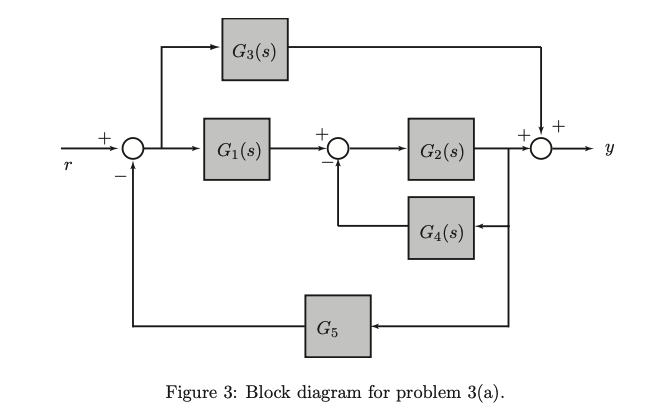
\includegraphics[width=300pt]{midterm_2012_q3.png}

Let the output after each junction be $J_1(s), J_2(s), J_3(s)$ respectively. Then we have

\begin{align*}
    Y(s) &= J_3(s) \\
    J_3(s) &= G_3(s) J_1(s) + G_2(s) J_2(s) \\
    J_2(s) &= G_1(s) J_1(s) - G_4(s) G_2(s) J_2(s) \\
    J_1(s) &= R(s) - G_5(s) G_2(s) J_2(s) \\
\end{align*}

\begin{align*}
    J_2(s) &= G_1(s) J_1(s) - G_4(s) G_2(s) J_2(s) \\
    J_2(s) -  J_2(s) G_4(s) G_2(s) &= G_1(s) J_1(s) \\
    J_2(s) (1 - G_4(s) G_2(s)) &= G_1(s) J_1(s) \\
    J_2(s) &= \dfrac{G_1(s)}{1 - G_4(s) G_2(s)} J_1(s) \\
\end{align*}

\begin{align*}
    J_1(s) &= R(s) - G_5(s) G_2(s) J_2(s) \\
    J_1(s) &= R(s) - \dfrac{G_1(s) G_5(s) G_2(s)}{1 - G_4(s) G_2(s)} J_1(s) \\
    J_1(s) + \dfrac{G_1(s) G_5(s) G_2(s)}{1 - G_4(s) G_2(s)} J_1(s) &= R(s) \\
    J_1(s) \left(1 + \dfrac{G_1(s) G_5(s) G_2(s)}{1 - G_4(s) G_2(s)} \right) &= R(s) \\
    J_1(s) &= \dfrac{R(s)}{1 + \dfrac{G_1(s) G_5(s) G_2(s)}{1 - G_4(s) G_2(s)}}  \\
\end{align*}

\begin{align*}
    Y(s) &= J_3(s) \\
    J_3(s) &= G_3(s) J_1(s) + G_2(s) J_2(s) \\
    Y(s) &= G_3(s) J_1(s) + G_2(s) J_2(s) \\
    Y(s) &= G_3(s) \left( \dfrac{R(s)}{1 + \dfrac{G_1(s) G_5(s) G_2(s)}{1 - G_4(s) G_2(s)}} \right) + G_2(s) \left( \dfrac{G_1(s)}{1 - G_4(s) G_2(s)} \right) \left( \dfrac{R(s)}{1 + \dfrac{G_1(s) G_5(s) G_2(s)}{1 - G_4(s) G_2(s)}} \right)
\end{align*}

\subsection{Question 4}

Consider the feedback system in Figure 4 with

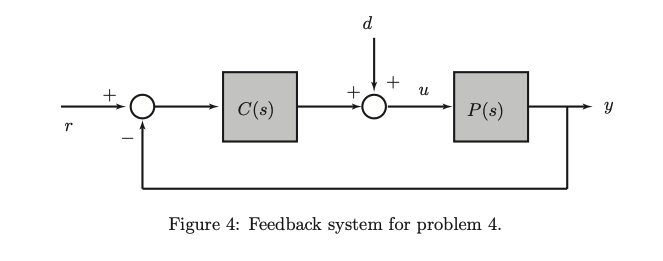
\includegraphics[width=300pt]{midterm_2012_q4.png}

\[ C = K_p + \dfrac{K_i}{s} \]
\[ P(s) = \dfrac{1}{2s + 1} \]

Where $K_p, K_I$ are real, constant, controller gains.

\subsubsection{a}

Find conditions on $K_p$, $K_I$ so that the output response, due to the reference input $r$, is underdamped.

The overall transfer function (ignoring $d$ for now bc we want to only consider the reference input $r$) is given by $G(s) = \dfrac{C(s) P(s)}{1 + C(s) P(s)}$ and we want to choose values so that the poles of this overall transfer function have a non-zero imaginary part. (i'm not sure how they'd want you to manually do this).

\subsubsection{b}

Suppose that we are given the following specifications for the transfer function from $R$ to $Y$:

\begin{enumerate}
    \item BIBO stability
    \item $T_s \leq 3$ for a step input
    \item Less than 10 percent overshoot for a step input
\end{enumerate}

Treating the closed-loop systema s a prototype second order system draw the region of allowable s-plane pole locations so that the system meets these specifications.

A rough sketch of the answer: all poles must be $< 0$ for it go be bibo stable. For settling time to be within a certain bound, the negative parts of all poles must be less than some small value. For less than a certain amount of overshoot, the zeta values of our poles must be greater than some value which puts another restrictions on the min/max values of the imaginary parts of our poles.

\subsubsection{c}

Choose values of $K_P$ and $K_I$ so that the specifications from part (b) are met. Comment on how the actual closed-loop system will respond given that it isn't actually a prototype second order system.

Not sure how to do, also long.

\subsubsection{d}

Using the values of $K_I$ and $K_P$ from part (c), find the steady-state output $y_{ss}(t)$ due to a unit step disturbance $d(t) = 1(t)$ when $r(t) = 0$.

The steady state output should be given by our value of $\mu$ from the transfer function, which can be computed after plugging in the values of $K_I$ and $K_P$ from part (c).

\end{document}
